\documentclass{article}

\usepackage{times}
\usepackage{geometry}
\geometry{a4paper,left=0.6cm,right=0.7cm,top=1.5cm,bottom=1cm,columnsep=0.8cm}

\usepackage{fontawesome}          % icônes de base seulement
\usepackage[hidelinks]{hyperref}
\usepackage{multicol}
\usepackage{tikz}
\usepackage{hyphsubst}
\usepackage{moresize}
\usepackage{hyphenat}
\usepackage{tabularx}
\usepackage{xcolor}
\usepackage{enumitem}
\usetikzlibrary{calc, positioning}
\newcolumntype{Y}{>{\RaggedRight\arraybackslash}X}

% icônes manquantes -> puce
\makeatletter
\@for\sym:=faBrain,faMicrochip,faHandshakeO,faTools,faNetworkWired,%
             faDatabase,faServer,faGit,faUsers,faComments,faCalendar,faGroup\do{%
  \@ifundefined{\sym}{\expandafter\newcommand\csname\sym\endcsname{\textbullet}}{}}
\makeatother

% couleurs
\definecolor{maincolor}{HTML}{f0fafc}
\definecolor{seccolor}{HTML}{ffffff}
\definecolor{gray}{HTML}{8c94a9}
\definecolor{sidetext}{HTML}{59cee5}

% bande latérale bleue
\usepackage{eso-pic}
\AddToShipoutPictureBG{%
  \begin{tikzpicture}[remember picture,overlay]
    \fill[maincolor] (current page.north west) rectangle
                     ([xshift=0.3\paperwidth] current page.south west);
  \end{tikzpicture}%
}

% listes
\setlist[itemize]{itemsep=-2pt,topsep=0pt,leftmargin=1.08cm}
\renewcommand{\labelitemi}{\textcolor{sidetext}{\footnotesize$\bullet$}}

\setlength{\parindent}{0pt}
\usepackage{paracol}
\columnratio{0.3}

\begin{document}
\pagestyle{empty}

\begin{paracol}{2}
% ────────────────────────────────────────
% Colonne gauche
% ────────────────────────────────────────
\color{sidetext}
\vspace*{-0.5cm}

\noindent
\begin{minipage}{\linewidth}
  \centering
  \begin{tikzpicture}
    \clip (0,0) circle (1.5cm) node[anchor=center]
      {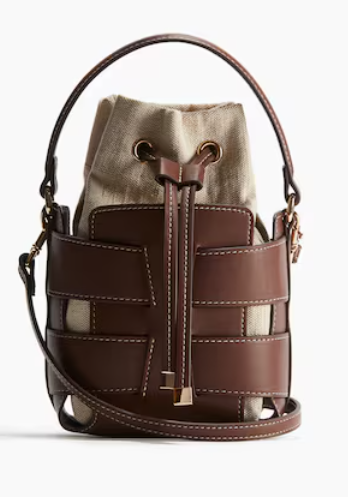
\includegraphics[width=3cm]{e8972633822c413e927ac1f850dfee3b.png}};
  \end{tikzpicture}

  \vspace{3mm}
  {\color{black}\LARGE \textbf{Pape Saliou Fall}}

  \vspace{1mm}
  {\large Ingénieur Data Scientist \& Développeur IA}

  \vspace{3mm}
  {\color{gray}\rule{\linewidth}{0.4pt}} \\
\end{minipage}

% ── Coordonnées
\begin{tabular}{@{}c l}
  \faPhone &
  \begin{tabular}[t]{@{}l@{}}
    {\color{gray}Téléphone} \\ 0753481453
  \end{tabular} \\
  \\
  \faLinkedin &
  \begin{tabular}[t]{@{}l@{}}
    {\color{gray}LinkedIn} \\
    \href{https://www.linkedin.com/in/pape-saliou-fall-43154a211/}{Mon LinkedIn}
  \end{tabular} \\
  \\
  \faMapMarker &
  \begin{tabular}[t]{@{}l@{}}
    {\color{gray}Adresse} \\ 95300 Pontoise \\ 
  \end{tabular} \\
  \\
  \faEnvelope &
  \begin{tabular}[t]{@{}l@{}}
    {\color{gray}Email} \\
    \href{mailto:papesalioufall2@gmail.com}{papesalioufall2@gmail.com}
  \end{tabular} \\
\end{tabular}

\vspace{2mm}
{\color{gray}\rule{\linewidth}{0.4pt}} \\

% ── Langues --------------------------------------------------------
{\color{black}{Langues}}

\vspace{2mm}
\begin{itemize}[leftmargin=*]
\item English - \textcolor{gray}{B2}
\item French - \textcolor{gray}{Native}\end{itemize}          % ← le placeholder va contenir \begin{itemize}…\end{itemize}

{\color{gray}\rule{\linewidth}{0.4pt}} \\

% ── Compétences ----------------------------------------------------
\vspace{2mm}
{\color{black}{Compétences Clés}}

\vspace{2mm}
\begin{itemize}[leftmargin=*]
\item Python
\item C
\item JavaScript
\item C++
\item R
\item SQL
\item PowerBI\end{itemize}              % ← idem, une vraie liste
\vspace{2mm}
{\color{gray}\rule{\linewidth}{0.4pt}} \\

% ── Centres d'intérêt
\vspace{2mm}
{\color{black}{Centres d’intérêt}}

\vspace{2mm}
\begin{itemize}[leftmargin=*]
\item Football
\item Swimming
\item Reading
\item Poetry
\end{itemize}     % ← simple itemize ou tabular

\vfill
~

% ────────────────────────────────────────
\switchcolumn
% Colonne droite
% ────────────────────────────────────────
\color{black}

% ── Profil
\textcolor{black}{\Large \textbf{Profil Professionnel}} \\[2pt]
Data Scientist passionné par la transformation de données complexes en solutions à forte valeur ajoutée, j’évolue aujourd’hui en CDI sur des projets d’IA de bout en bout. Mes expériences m’ont permis de maîtriser l’ensemble du cycle de vie d’un modèle, de l’ingestion de données à la mise en production cloud. Autonome, curieux et orienté résultats, je cherche désormais à relever de nouveaux défis dans un environnement où l’innovation et la collaboration sont centrales. \\[8pt]

% ── Expérience
\textcolor{black}{\Large \textbf{Expérience Professionnelle}} \\[2pt]

\colorbox{maincolor}{%
  \begin{minipage}{\linewidth}
    \textbf{Data Scientist \& Développeur IA} \\ Prepaya \\ 01/2024 - Présent
    \begin{itemize}
      \item Conçu et déployé une plateforme d’IA end-to-end (Python/JavaScript) pour automatiser l’analyse de séries chronologiques. \item Implémenté des modèles Machine \& Deep Learning avec Scikit-learn et TensorFlow, améliorant la précision des prévisions. \item Industrialisé les modèles via API Flask sur Heroku/PostgreSQL, réduisant le temps de mise en production.
    \end{itemize}
  \end{minipage}}

\vspace{3mm}


\colorbox{maincolor}{%
  \begin{minipage}{\linewidth}
    \textbf{Apprenti Risk Analyst \& Data Scientist} \\ AXA XL (Groupe AXA) \\ 12/2022 - 12/2023
    \begin{itemize}
      \item Automatisé la collecte de données financières avec Python et VBA, divisant par deux le temps de reporting. \item Développé des tableaux de bord Power BI pour la facturation, offrant une visibilité temps réel aux équipes finance et gestion. \item Créé une application prédictive des sinistres (Python/SQL) augmentant la précision d’estimation du risque pour les clients.
    \end{itemize}
  \end{minipage}}

\vspace{3mm}


\colorbox{maincolor}{%
  \begin{minipage}{\linewidth}
    \textbf{Apprenti Data Scientist} \\ Prepaya \\ 09/2021 - 08/2022
    \begin{itemize}
      \item Développé des modèles NLP (T5, BERT) générant automatiquement des formulaires clients et réduisant le temps de traitement. \item Mis en place une analyse de sentiment sur les retours utilisateurs, fournissant des insights pour améliorer la satisfaction. \item Automatisé la collecte web avec BeautifulSoup et Selenium afin d’enrichir le corpus de données et d’améliorer les performances modèles.
    \end{itemize}
  \end{minipage}}   % ← blocs \colorbox{maincolor}{\begin{minipage}…}

\vspace{8mm}

% ── Formation
\textcolor{black}{\Large \textbf{Formation}} \\[2pt]

    \begin{tabularx}{\linewidth}{@{}c X@{}}
    \textcolor{sidetext}{\faGraduationCap} &
    \textbf{Master 2 Data Science} \\
    & Sorbonne Université \\
    & \begin{itemize}[leftmargin=*]
  \item Approfondissement en analyse de données, Machine Learning et Deep Learning. \item Cours sur modèles de séries temporelles, apprentissage statistique et calcul parallèle. \item Projets pratiques de modélisation et visualisation de données complexes.
\end{itemize} \\
    & \textit{09/2021 - 03/2022}
    \end{tabularx}
           % ← lignes tabular par diplôme

\end{paracol}
\end{document}

